\section{液化}\label{sec:4-4}

物质从气态变成液态的现象叫做\textbf{液化}。
正象凝固是熔解的相反过程一样,液化是汽化的相反过程.

\begin{wrapfigure}{r}{7cm}
    \centering
    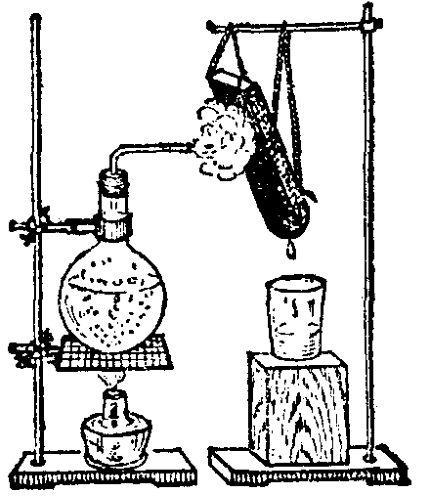
\includegraphics[width=6cm]{../pic/czwl2-ch4-8}
    \caption{水蒸气温度降低凝结成水}\label{fig:4-8}
\end{wrapfigure}


让水蒸气喷到一个冷的物体上,水蒸气就变成水(图 \ref{fig:4-8})。
烧水时看到的“白气” 就是水蒸气温度降低凝结成的小水珠。
可见,降低温度,可以使水蒸气液化。

实验表明,所有的气体,在温度降低到足够低的时候,都可以液化。

气体的液化温度跟压强有关系。
例如,水蒸气在 1 标准大气压下,液化温度是 100 ℃;
在 3 标准大气压下,要在 134 ℃ 才凝结成水。
可见,气体的压强越大,它的液化温度越高。

一些通常情况下是气体状态的物质,在大气压下要在很低的温度才能液化;
如果采用增大压强的办法,在较高的温度下就可以使它们液化。
例如,许多地方使用的液化石油气,就是在常温下用增大压强的方法,
使它成为液体储存在钢罐里的。

跟液体在汽化时要吸收热量相反,气体在液化时要放出热量。
被水蒸气烫伤往往比被开水烫伤还严重,就是因为水蒸气液化时放出了热量的缘故。

实验表明,某种物质在从气体变成同温度的液体时放出的热量,
等于它在这一温度下,由液体变成气体时吸收的热量。
这就是说,单位质量的某种物质,在从气体变成同温度的液体时放出的热量,
等于它在这一温度时的汽化热。
例如,1 克 100 ℃ 的水蒸气在凝结成 100 ℃ 的水时,放出的热量就是 539 卡。

在自然界中,我们可以看到水蒸气凝结成水的例子。
白天气温较高,地球表面的水大量蒸发,空气中有较多的水蒸气;
夜间气温较低,空气中的水蒸气就在草木、石块等上面凝成小水珠,这就是露。
如果空气中有较多的浮尘,空气中的水蒸气就凝结在这些浮尘上面,这就是雾。


\section*{阅读材料:致冷设备}

我们知道,液体汽化时有致冷作用,致冷设备就是根据这种作用制成的。

常用的致冷设备主要由压气机、冷凝器和蒸发器三部分组成(图 \ref{fig:4-9})。
\begin{figure}[htbp]
    \centering
    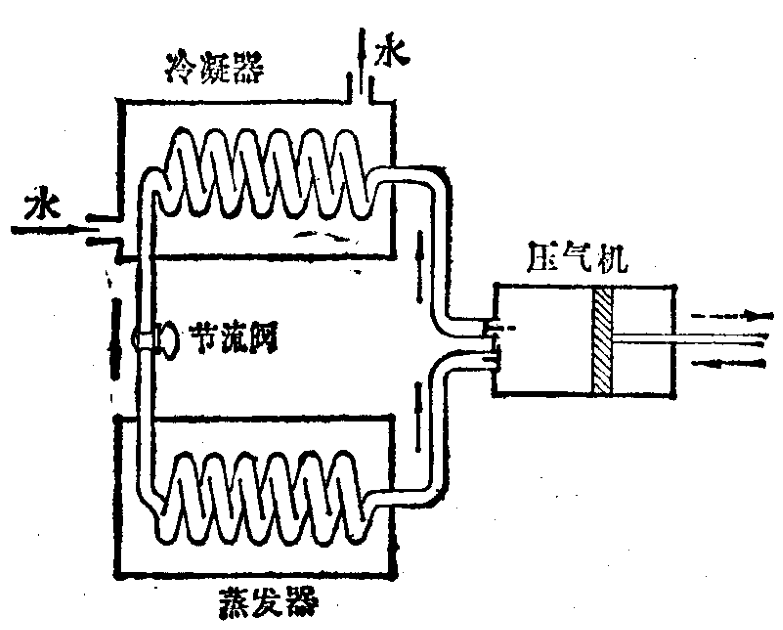
\includegraphics[width=0.6\textwidth]{../pic/czwl2-ch4-9}
    \caption{致冷设备的示意图}\label{fig:4-9}
\end{figure}
其中的工作物质是容易由气态变成液态和由液态变成气态的物质,常用的有氨及氟氯烷等。
压气机产生大约 10 标准大气压的压强,把气态氨压入冷凝器的管里,这时氨变了液体。
氨在液化时放出的热量被流动的冷水吸收并带走。
冷凝器的管里的液态氨通过节流阀缓慢地进入蒸发器的管里。
由于压气机不断地从蒸发器的管里吸走气体,这个管里的压强就比较低,于是液态氨在蒸发器的管里迅速汽化。
在汽化中从管外的食盐水里吸取热量,使食盐水的温度降低。
生成的氨气又被压气机抽走,压入冷凝器,这样氨可以循环使用。
温度降低后的食盐水可作为致冷剂用来制冰、冷却食品或降低夏季房间里的气温。
在用于降低房间里的气温时,通常不用食盐水而是直接使空气从蒸发器管子的周围流过而得到冷却,
再把冷却后的空气送到房间里去。


